\documentclass{../../../ExampleProblem}
\usepackage{../../../mathshortcuts}


\title{Beam Analysis}
\author{Brian Chevalier}
\subtitle{Beam Analysis}
\coursenum{CEE421}
\coursetitle{Concrete Design}
\university{gitMechanics}
\date{\today}

\begin{document}

\problemstatement
{Select the area of steel, $A_s$, cross section width, $b$, and effective depth $d$ for the cross section shown.}
{
	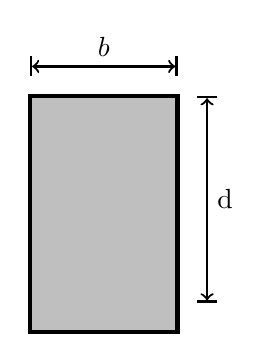
\begin{tikzpicture}[scale=0.75]
		\draw[ultra thick,fill=lightgray] (0,0)rectangle(2.5,4);
		\draw[thick,|<->|] (0,4.5)--node[above]{$b$}(2.5,4.5);
		\draw[thick,|<->|] (3,0.5) --node[right]{d}(3,4);
		\poi{0.5,0.5}
		\poi{1,0.5}
		\poi{1.5,0.5}
		\poi{2,0.5}
	\end{tikzpicture}
}


\section{Solution Strategy}
To solve this problem we must start with the basic design relationship, assume the steel is yielding, 


We start with the basic design relationship $\phi M_n \geq M_u$. The nominal moment can be substituted in for the moment when taking moments about the concrete compressive force.




\end{document}

